\documentclass[../thesis.tex]{subfiles}
% Separate preamble for this subfile. This preamble is loaded last, so one can override various functions before \begin{document}

% Better comment extension for Vscode colors these comments differently
% Normal comment color
% * Important information
% ! ALERT
% ? Question
% TODO stuff to do
% // this is strikethrough


\begin{document}

Before tackling spectral sets in higher dimensions, we first emphasize the importance of \cref{eq:zero_set_equation} and generalize it to higher dimensions. 
\begin{lemma}\label{lem:zero_set_jp_1_5}
    Let $\Omega=I^d$. The zero-set for the function
    \begin{equation*}
        F_{\Omega} (z):= \int_\Omega e^{2 \pi i \braa{z,t}} dt
    \end{equation*}
    is the set
    \begin{equation*}
        \Zstroke_{I^d} = \braqMed{ z = \brac{z_1,\dots,z_d}\in \C^d \setminus \braqMed{0} : \exists \space j \in \braqMed{1,\dots, d} \text{ such that } z_j \in  \intnozero}
    \end{equation*}
\end{lemma}

\begin{example}
    The zero-set for $F_{\Omega}$ when $d=1$ is the following
    \begin{equation*}
        %\Zstroke_{I} = \braqMed{ z \in \C \setminus \braqMed{0} : \exists \space z \in  \intnozero} = \braq{z: z \in \intnozero}
        \Zstroke_{I} = \braq{z: z \in \intnozero} \qedhere
    \end{equation*}
\end{example}

\begin{proof}[Proof of  \cref{lem:zero_set_jp_1_5}]
    Given a vector $z \in C^d$ we can factor $F_{\Omega}$ for $\Omega = I^d$ as follows
    \begin{align*}
        F_{I^d} (z) &= \int_{I^d} e^{2 \pi i \braa{z,t}} dt\\
        &= \int_{I^d} e^{2\pi i  (z_1 t_1 + \dots +z_d t_d)} dt\\
        &= \int_{I^d} e^{2\pi i z_1 t_1}  \cdots e^{2\pi i z_d t_d}  dt\\
        &= \int_{I} e^{2\pi i z_1 t_1} \int_{I} e^{2\pi i z_2 t_2}  \cdots \int_{I} e^{2\pi i z_d t_d}  dt_1 dt_2\dots dt_d\\
        &=\prod_{j=1}^d \int_I e^{2\pi i z_j t_j} dt_j
    \end{align*}
    If $z=0$, then $e^{2\pi i z_j t_j} = 1$ and
    \begin{align*}
        F_{I^d} (0) = \prod_{j=1}^d \int_I 1 \space dt_j = \brac{\mes{I}}^d = 1.
    \end{align*}
    Thus we must have $z\in \C^d\setminus\braq{0}$. Assume now that $z\neq 0$. Integration yields
    \begin{align*}
        F_{I^d} (z) = \prod_{j=1}^d \frac{e^{2 \pi i z_j} -1}{2 \pi i z_j}.
    \end{align*}
    This equation is zero whenever at least one element $z_j\in \intnozero$ using that the exponential equals one in this case, and also not to get an undefined fraction. Thus, the zero set for $F_{I^d}$ is $\Zstroke_{I^d}$ which completes the proof.
\end{proof}

\begin{remark}
    Given a spectral pair $(I^d,\Lambda)$, consider the set
    \begin{equation*}
        \Lambda - \Lambda = \braqMed{\lambda-\lambda' : \lambda,\lambda' \in \Lambda}.
    \end{equation*}
    %! Sjekk opp denne med lydlog
    It follows that the spectral pair property is equivalent to the non-zero elements of $\Lambda - \Lambda$ being contained in the zero-set of $F_{\Omega}$. More specifically, if $(I^d,\Lambda)$ is a spectral pair, then
    \begin{equation*}
        \Lambda - \Lambda \subset \Zstroke_{I^d} \cup \braq{0}
    \end{equation*}
    This follows immediately from the observation that
    \begin{equation*}
        \braaMed{e_{\lambda},e_{\lambda'} }_{L^2(I^d)} = \int_\Omega e^{2 \pi i \braa{(\lambda-\lambda'),t}} dt = F_{\Omega} (\lambda-\lambda'),
    \end{equation*}
    %which is zero whenever $\lambda \neq \lambda'$, that is $\lambda-\lambda'\neq 0$, which imply $\lambda-\lambda' \in \Z_{I^d}$
    which is zero whenever $\lambda \neq \lambda'$, which implies $\lambda-\lambda' \in \Zstroke_{I^d}$
\end{remark}

\begin{example}
    Observe that for $\Lambda=\Z$, the non-zero elements of $\Lambda - \Lambda$ is simply $\intnozero$. Clearly
    \begin{equation*}
        \intnozero \subset \Zstroke_{I} \cup \braq{0} = \Z
    \end{equation*}
\end{example}

%! BEGYN HER
%* —————————————————————————————————————


In \cite{jorgensenSpectralPairsCartesian2001}, Pedersen and Jorgensen present a way of constructing spectral pairs in higher dimensions from spectral pairs in lower dimensions. 

\begin{theorem}[Construction of spectra]\label{thrm:construction_spectra}
    Let $\brac{\Omega_1,\Lambda_1}$ be a spectral pair in $\R^{d_1}$, and let $\Omega_2$ be a set of positive finite measure in $\R^{d_2}$. Suppose for each $\lambda_1 \in \Lambda_1$ that $\lambfunc$ is a discrete subset of $\R^{d_2}$ such that $\brac{\Omega_2,\lambfunc}$ is a spectral pair. If 
    \begin{equation*}
        \Lambda = \braq{\brac{\lambda_1, \lambda_2}: \lambda_1\in \Lambda_1, \lambda_2 \in \lambfunc} 
    \end{equation*}
    then $\brac{\Omega_1\times\Omega_2, \Lambda}$ is a spectral pair in $\R^{d_1+d_2}$ dimensions. 
\end{theorem}

\begin{remark}
    It can be helpful to think of $\lambfuncNoVar$ as a function that assigns a discrete subset in $\R^{d_2}$ to each $\lambda_1$-value such that $\brac{\Omega_2,\lambfunc}$ is itself a spectral pair. However, $\lambfunc$ should never be considered anything other than a set of points. 
\end{remark}

\begin{proof}
    Given $\Lambda$ as constructed in \cref{thrm:construction_spectra}, we start by showing that the set of exponentials $E(\Lambda)$ is orthogonal in $L^2\brac{\Omega_1 \times \Omega_2}$. For two elements $e_\lambda,e_{\lambda'} \in E(\Lambda)$ we have %the following inner product %Note that $t$ denotes the vector $(t_1,t_2)$ where $t_1 in \Omega_1$ and $t_2 \in \Omega_2$
    \begin{align*}
        \braa{e_\lambda,e_{\lambda'}}_{L^2\brac{\Omega_1 \times \Omega_2}} 
        &= \int_{\Omega_1} \int_{\Omega_2} e_{\lambda}(t) \overline{e_{\lambda'}(t)} dt_2 dt_1\\ 
        &= \int_{\Omega_1} \int_{\Omega_2} e^{2\pi i \braa{\lambda, t} } e^{-2\pi i  \braa{\lambda', t}} dt_2 dt_1\\ 
        &= \int_{\Omega_1} \int_{\Omega_2} e^{2\pi i \brac{\lambda_1 t_1+\lambda_2 t_2}} e^{-2\pi i\brac{\lambda_1' t_1+\lambda_2' t_2}} dt_2 dt_1\\ 
        &= \int_{\Omega_1} \int_{\Omega_2} e^{2\pi i \brac{\lambda_1- \lambda_1'}t_1} e^{2\pi i \brac{\lambda_2 - \lambda_2'}t_2} dt_2 dt_1\\ 
        &= \int_{\Omega_1} e^{2\pi i  \brac{\lambda_1- \lambda_1'}t_1} \bracMed{\int_{\Omega_2}  e^{2\pi i \brac{\lambda_2 - \lambda_2'}t_2} dt_2} dt_1.
    \end{align*}
    If $\lambda_2 \neq \lambda_2'$, then as $\lambda_2, \lambda_2' \in \lambfunc$ the inner integral will be zero from the fact that $\brac{\Omega_2, \lambfunc}$ is a spectral pair. Conversely, if $\lambda_2 = \lambda_2'$ the resulting integral will factor as % THE inner integral will be equal to $\mes{\Omega_2}$, and the resulting integral will be
    \begin{align*}
        = \mes{\Omega_2} \int_{\Omega_1} e^{2\pi i  \brac{\lambda_1- \lambda_1'}t_1} dt_1.
    \end{align*}
    Now, if one assumes $\lambda_1 \neq \lambda_1'$, then as both $\lambda_1, \lambda_1' \in \Lambda_1$ the integral will be zero from the fact that $\brac{\Omega_1, \Lambda_1}$ is a spectral pair. However, if $\lambda_1 = \lambda_1'$, observe that we have the case where $\lambda = \lambda'$, and
    \begin{align*}
        \braa{e_\lambda, e_\lambda}_{L^2\brac{\Omega_1 \times \Omega_2}}
        &= \int_{\Omega_1} \int_{\Omega_2} e_{\lambda}(t) \overline{e_{\lambda}(t)} dt_2 dt_1
        =\int_{\Omega_1} \int_{\Omega_2} |e^{2 \pi i \braa{\lambda, t}}|^2 dt_2 dt_1
        = \int_{\Omega_1} \int_{\Omega_2} |1|^2 dt_2 dt_1\\
        &= \mes{\Omega_2}\mes{\Omega_1} \neq 0
    \end{align*}
    To show that $E(\Lambda)$ is complete in $L^2(\Omega_1 \times \Omega_2)$, let $f\in L^2\brac{\Omega_1 \times \Omega_2}$ and assume it is orthogonal to $\spn{E(\Lambda)}$. For all $e_\lambda \in E(\Lambda)$ the inner product is
    \begin{align*} % REMEMBER t is a vector, i.e t=(t_1,t_2)
        \braa{e_\lambda,f}_{L^2\brac{\Omega_1 \times \Omega_2}}
        &= \int_{\Omega_1} \int_{\Omega_2} e_\lambda(t) \overline{f(t)} dt_2dt_1 \\
        &= \int_{\Omega_1} \int_{\Omega_2} e^{2\pi i  (\lambda_1 t_1 + \lambda_2 t_2)} \overline{f(t_1,t_2)} dt_2 dt_1 \\
        &= \int_{\Omega_1} e^{2 \pi i \lambda_1 t_1} \int_{\Omega_2}e^{2 \pi i \lambda_2 t_2} \overline{f(t_1,t_2)} dt_2 dt_1
        %&= 0
    \end{align*}
    If we fix $\lambda_2$, we denote the inner integral by \SigridComment{Fiksere $\lambda_2$ er unødvendig? må ikke da F, være en funksjon av $\lambda_2$ også?}
    \begin{equation}\label{eq:inner_eq}
        F(t_1) := \int_{\Omega_2} e^{2 \pi i \lambda_2 t_2} \overline{f(t_1,t_2)} dt_2,
    \end{equation}
    and note that $F\in L^2(\Omega_1)$. We thus have % This allows us to rewrite our initial inner product into
    \begin{equation*}%\label{eq:outter_eq}
        \braa{e_{\lambda}, f}_{L^2(\Omega_1\times \Omega_2)} = \int_{\Omega_1} e^{2 \pi i \lambda_1 t_1} F(t_1) dt_1 = \braa{e_{\lambda_1}, F}_{L^2(\Omega_1)} = 0, \quad \text{ for all } \lambda_1 \in \Lambda_1 .
    \end{equation*}
    Using the fact that $E(\Lambda_1)$ is complete in $L^2(\Omega_1)$, we have from \cref{lem:ONB_alternative_def} that $F(t_1)=0$ for almost every $t_1 \in \Omega_1$. Now as we must have \labelcref{eq:inner_eq} equal to zero, observe that since $\lambda_2$ was arbitrarily, and we know that $E(\lambfunc)$ is complete in $L^2(\Omega_2)$, then using \cref{lem:ONB_alternative_def} again implies that $f=0$ a.e. Thus, $E(\Lambda)$ is complete in $L^2\brac{\Omega_1 \times \Omega_2}$ which finalizes the proof.
    %Using the fact that $E(\Lambda_1)$ is complete in $L^2(\Omega_1)$, we have from \cref{lem:ONB_alternative_def} and almost all $t_1 \in \Omega_1$, that the only element in $L^2(\Omega_1)$ that results in $\braa{e_{\lambda_1}, F} = 0$ for all $e_{\lambda_1} \in E(\Lambda_1)$ is the zero-element $F=0$. Now as we must have \cref{eq:inner_eq} equal to zero, observe that as we fixed $\lambda_2$ arbitrarily, and we know that $E(\Lambda_2)$ is complete in $L^2(\Omega_2)$, then the same lemma also implies $f=0$. Thus, $E(\Lambda)$ is complete in $L^2\brac{\Omega_1 \times \Omega_2}$ which finalizes our proof.
    %For almost all $t_1 \in \Omega_1$ \cref{eq:outter_eq}
\end{proof}

Let us now give some examples using \cref{thrm:construction_spectra} to illustrate its ease of use and newfound flexibility. 
\begin{example}\label{exmp:first_construction}
    Let $\brac{\Omega_1,\Lambda_1}=\brac{I, \Z}$, which we know is a spectral pair in dimension $d_1=1$. Clearly $\brac{\Omega_2,\lambfunc}$ is also a spectral pair in dimension $d_2=1$ if $\Omega_2=I$ and $\lambfunc = \Z$ for all $\lambda_1 \in \Lambda_1$. Now, letting 
    \begin{equation}\label{eq:first_construction}
        \Lambda  = \braq{\brac{\lambda_1,\lambda_2}: \lambda_1 \in \Z, \lambda_2 \in \Z },
    \end{equation}
    it follows directly from \cref{thrm:construction_spectra} that $\brac{I^2, \Lambda}$ is a spectral pair in $1+1=2$ dimensions.
\end{example}

Recall our unproven \cref{lem:z_d_in_higer_d}. It is easy to see that applying \cref{thrm:construction_spectra} $d$ times will provide a proof of this result. \cref{exmp:first_construction} is an example of a lattice spectrum, but the increase in dimension allows for more flexibility in that we can also construct spectra that are not lattices. For instance, we can have the spectrum given by 
%This becomes evident when looking at FIGUREXX, which illustrates the grid-like pattern of a lattice. 
\begin{align}\label{eq:single_shift_func}
    \lambfunc = \begin{cases}        
        \Z & \text{for all } \lambda_1 \in \Lambda_1\setminus\braq{\lambda'}\\        
        \Z+\beta & \text{for } \lambda=\lambda',\text{ where } \beta \in \mathbb{R}   
    \end{cases}
\end{align}
for the two spectral pairs $\brac{I,\Z}$ and $\brac{I,\lambfunc}$ which is illustrated in \cref{fig:single_shift_vertical} with $\beta = 0.5$. Furthermore, we can shift on any number of the vertical axes, not just the one, and we can shift them with different amounts. In this case, we can have the spectrum given by \SigridComment{Begrense oss til kun skift mindre enn 1, og nevne at de kan være høyere, men det har ikke noe å si, eller innkludere skift på $15$. Nevner ikke noe om dette tidligere tror jeg}
\begin{align}\label{eq:multiple_shit_func}
    \lambfunc = \begin{cases}
        \vdots\\        
        \Z+0 & \text{for } \lambda_1 = -1 \in \Lambda_1\\
        \Z+0.3 & \text{for } \lambda_1 = \text{\space\space\space} 0 \in \Lambda_1\\
        \Z+0.8 & \text{for } \lambda_1 = \text{\space\space\space} 1 \in \Lambda_1\\
        \Z+0.5 & \text{for } \lambda_1 = \text{\space\space\space} 2 \in \Lambda_1\\
        \Z+0.9 & \text{for } \lambda_1 = \text{\space\space\space} 3 \in \Lambda_1\\
        \Z-0.3 & \text{for } \lambda_1 = \text{\space\space\space} 4 \in \Lambda_1\\
        \vdots
    \end{cases}
\end{align}
for the two spectral pairs $\brac{I,\Z}$ and $\brac{I,\lambfunc}$ which is illustrated in \cref{fig:multiple_shift_vertical}. Moreover, we can, in addition to the individual vertical shifts given by $\lambfunc$ in \labelcref{eq:multiple_shit_func}, also shift our other spectral pair $\brac{I,\Z}$ with, for example, $\alpha = 0.4$ as illustrated in \cref{fig:multiple_shift_horizontal}. At last, these shifts will also be accurate in the opposite direction by flipping the notation order, meaning $\Lambda_1$ is on the vertical axis, and $\lambfunc$ is on the horizontal axis.

%! FIGURE INPUT



\begin{figure}[t]%h!
    \centering
    \begin{subfigure}{.47\textwidth}
        \centering
        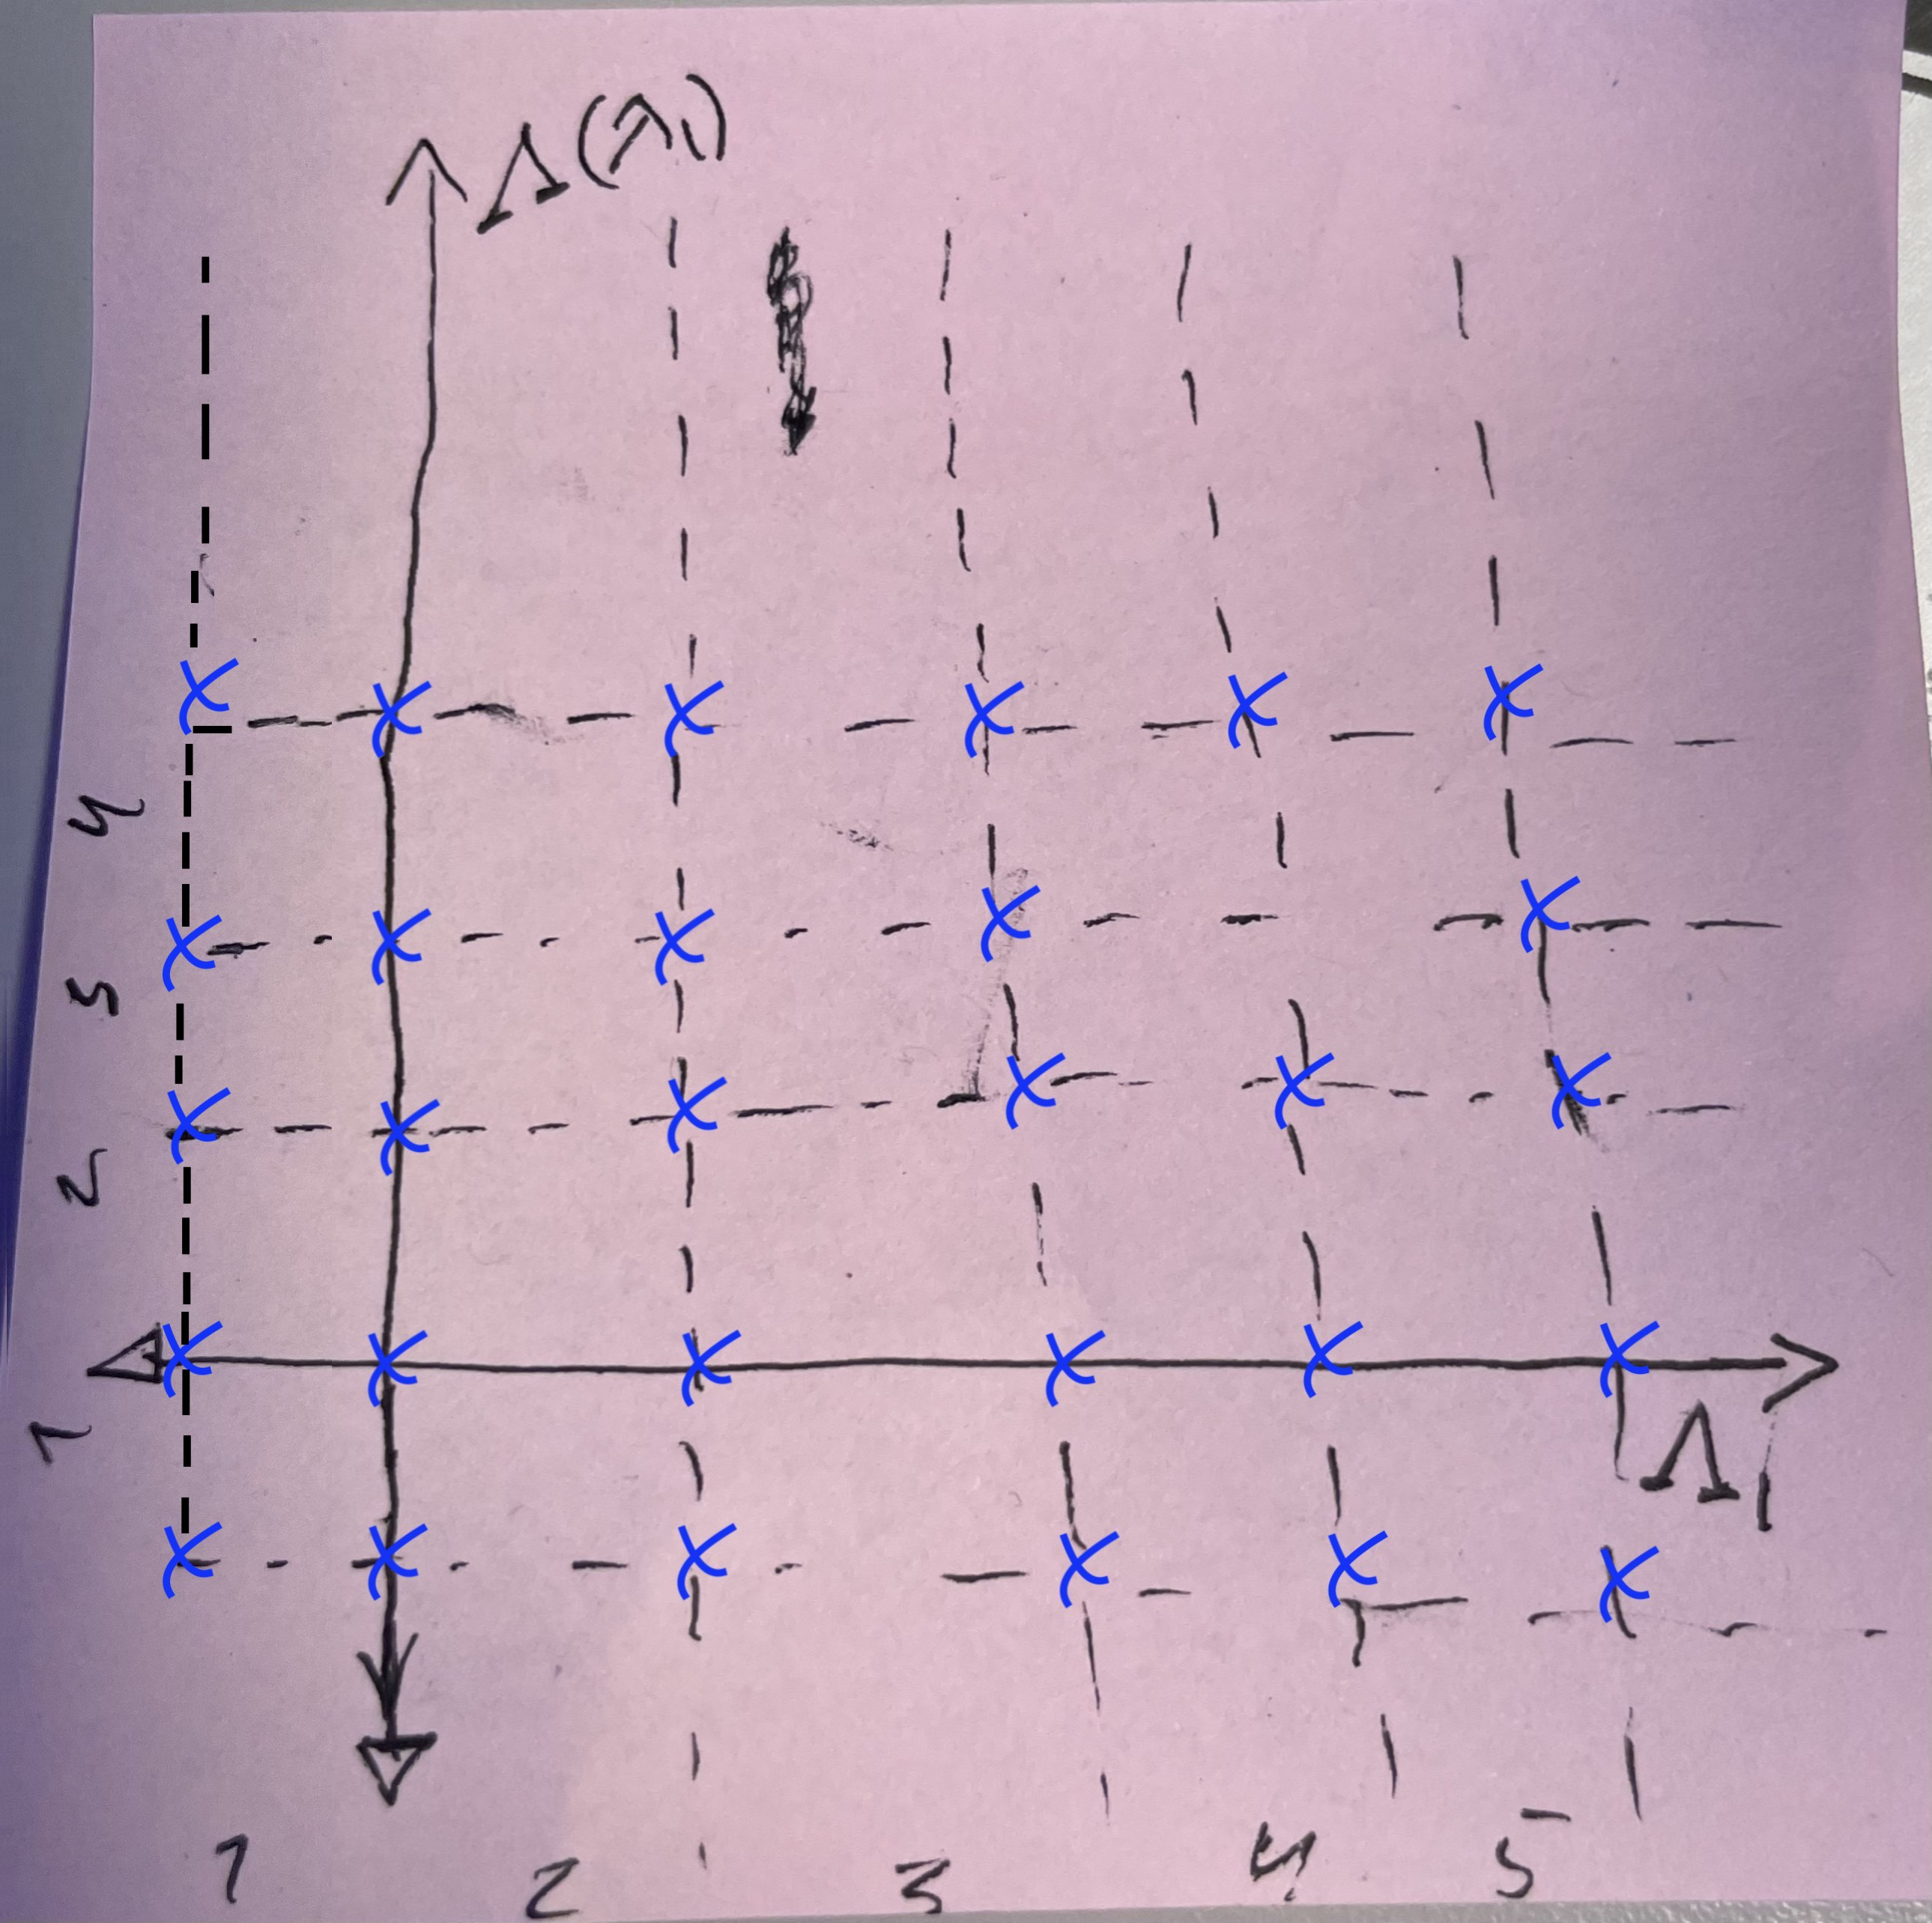
\includegraphics[width=0.9\linewidth]{spec_no_shift.jpg}
        \caption{Lattice spectra}
        \label{fig:lattice_spectra}
    \end{subfigure}\quad
    \begin{subfigure}{.47\textwidth}
        \centering
        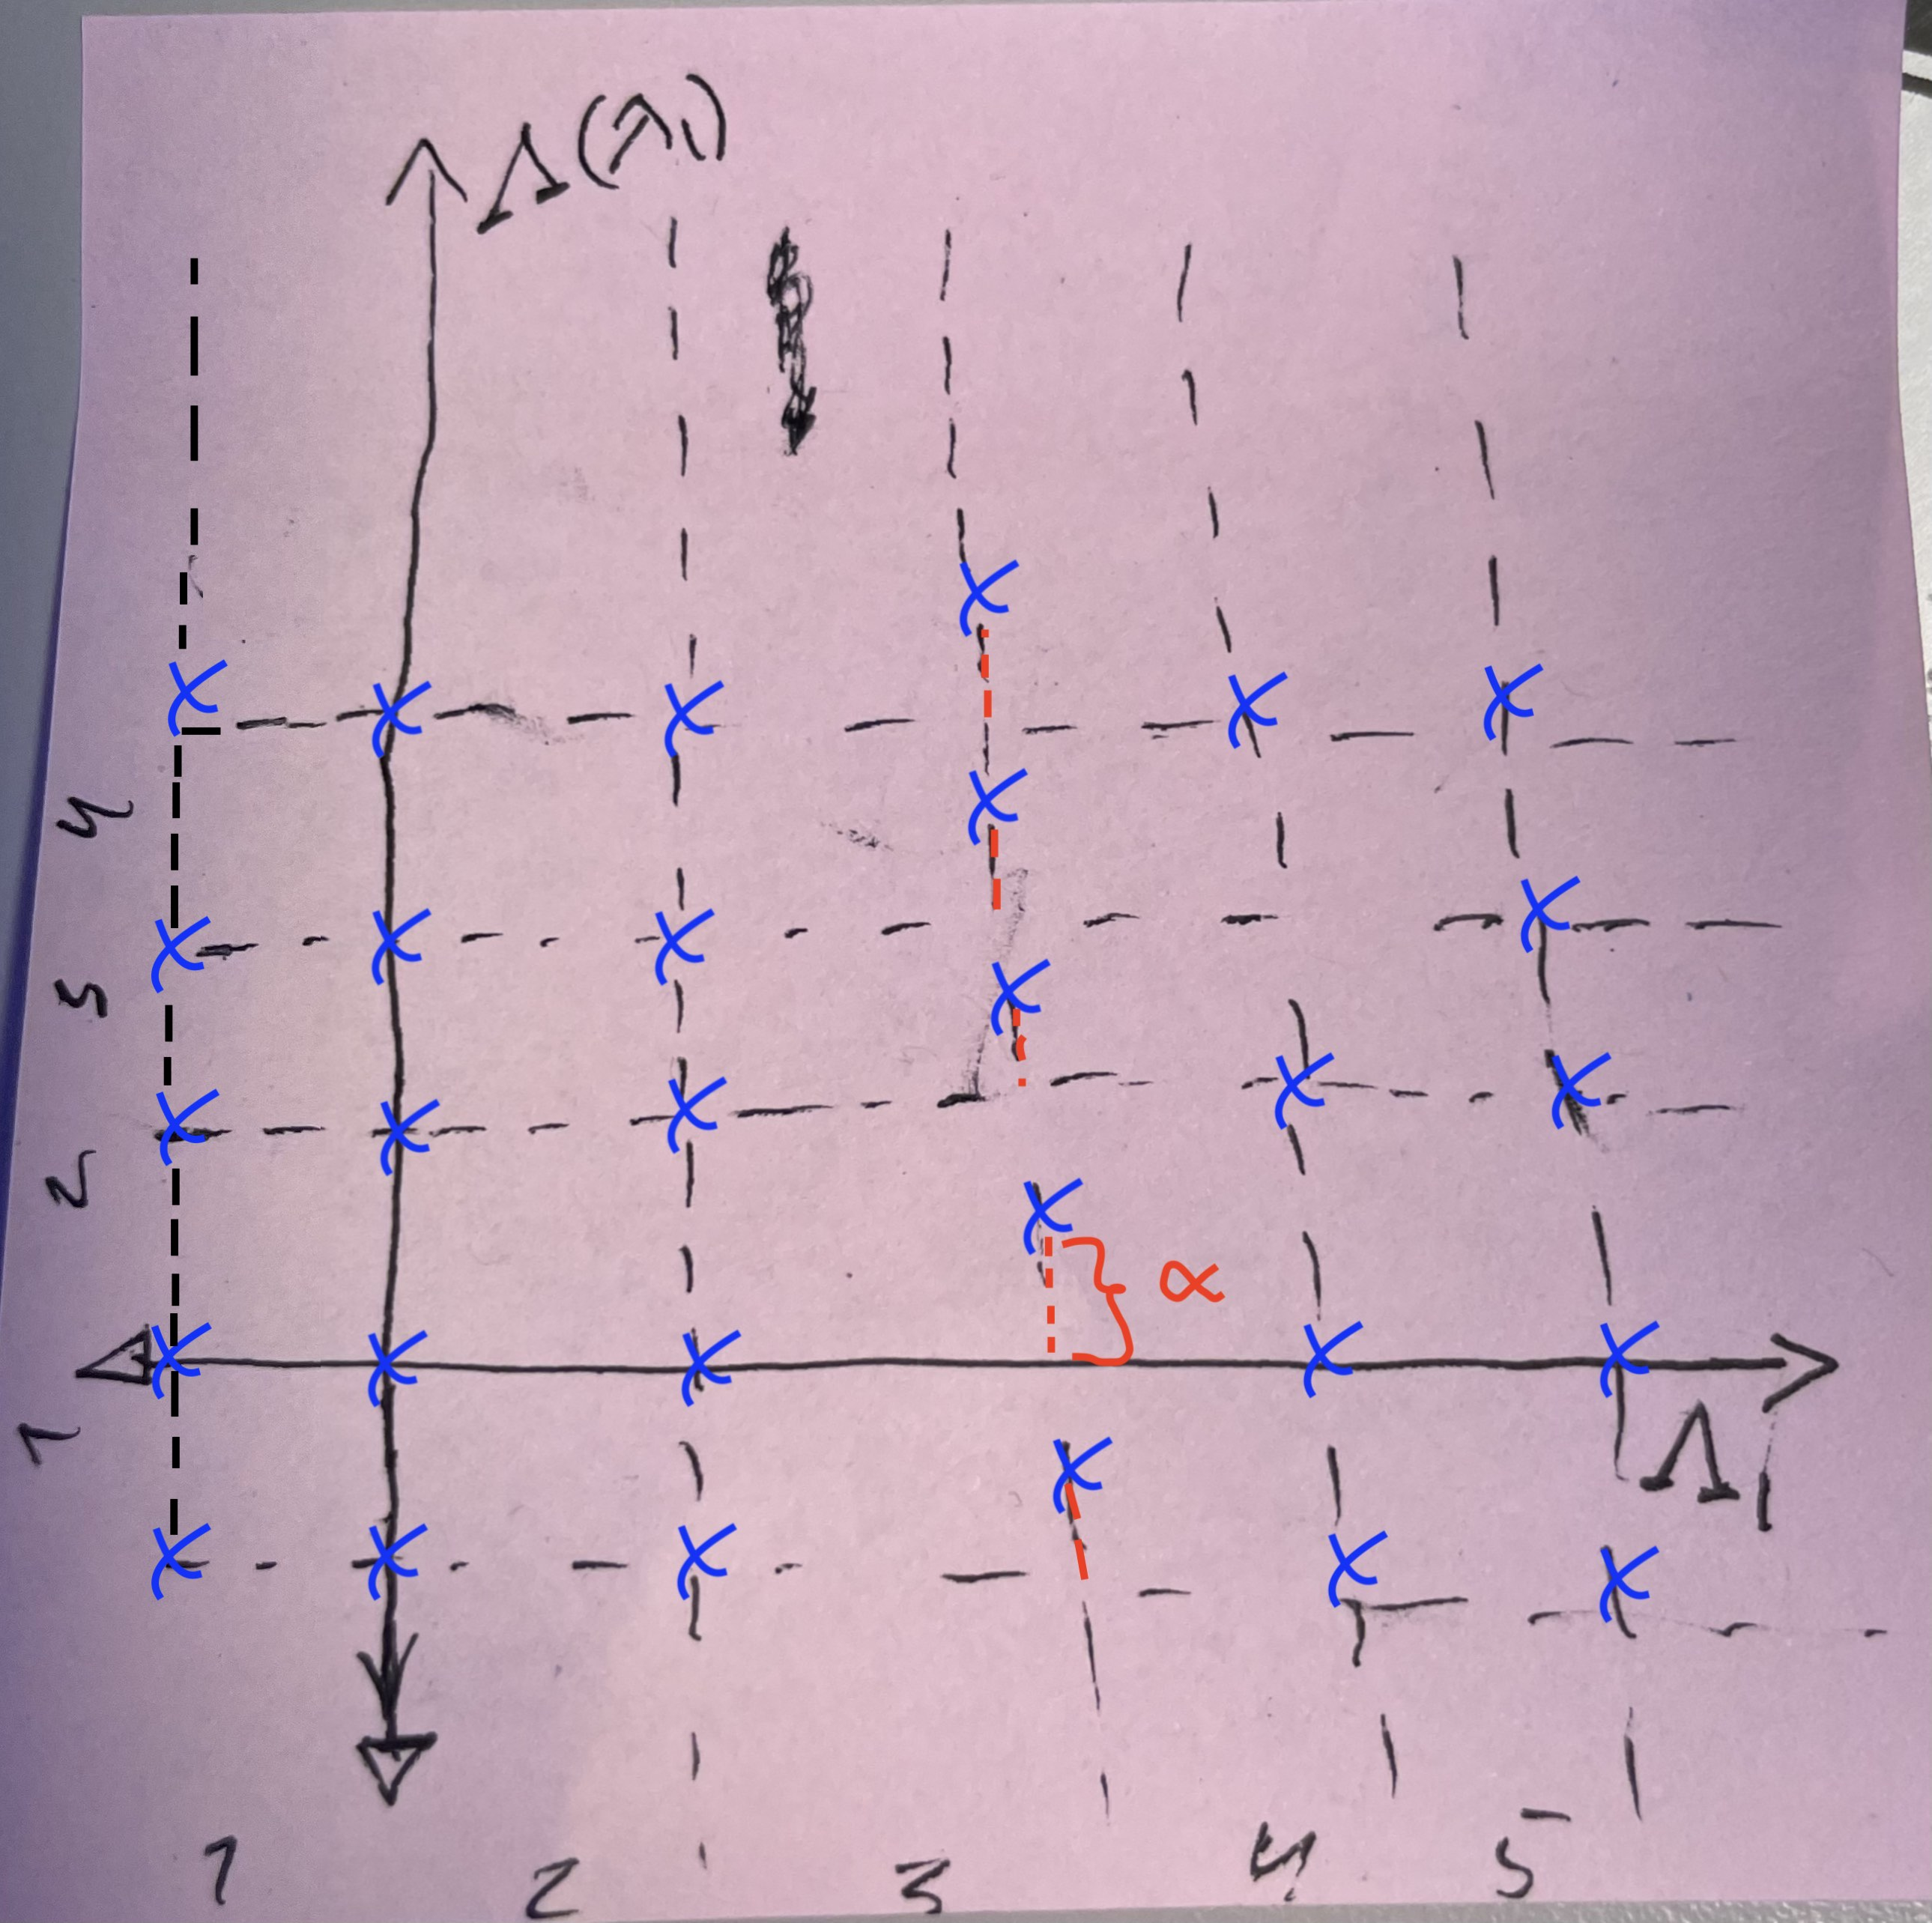
\includegraphics[width=0.9\linewidth]{spec_single_shift.jpg}
        \caption{Single shift vertical}
        \label{fig:single_shift_vertical}
    \end{subfigure}\\
    \begin{subfigure}{.47\textwidth}
        \centering
        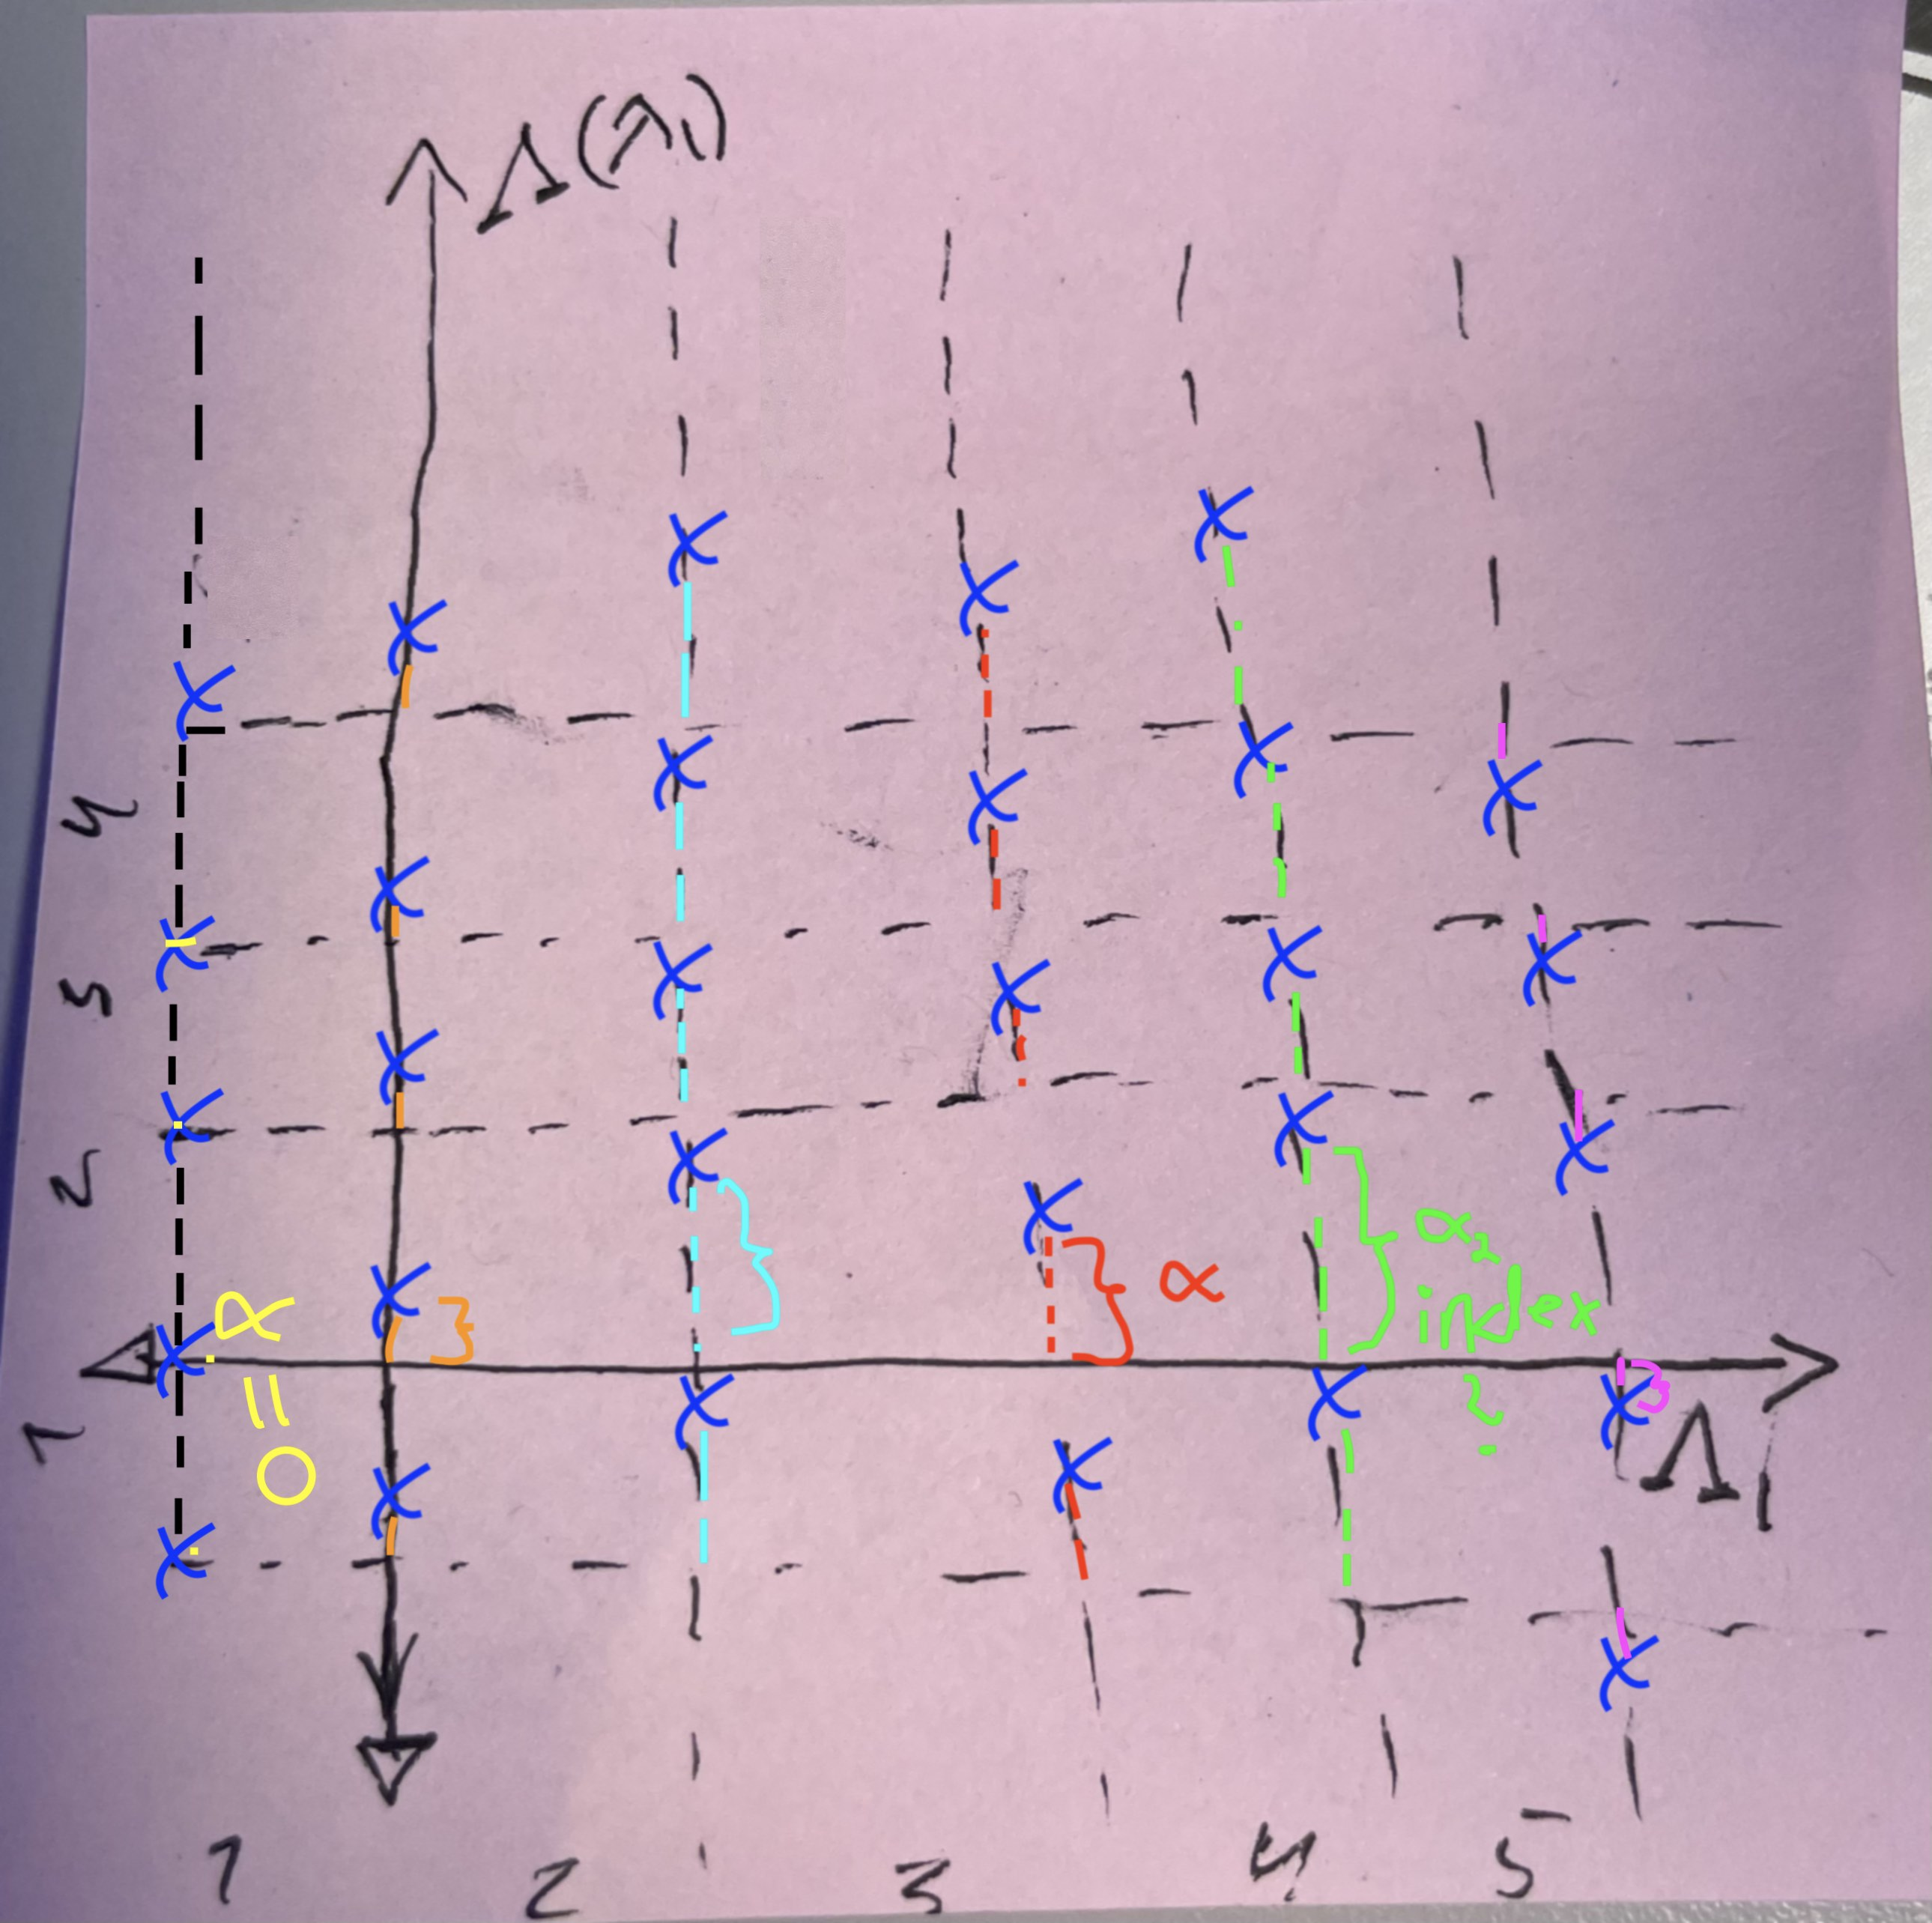
\includegraphics[width=0.9\linewidth]{multiple_shift_left_zero.jpg}
        \caption{Multiple individual shifts vertical}
        \label{fig:multiple_shift_vertical}
    \end{subfigure}\quad
    \begin{subfigure}{.47\textwidth}
        \centering
        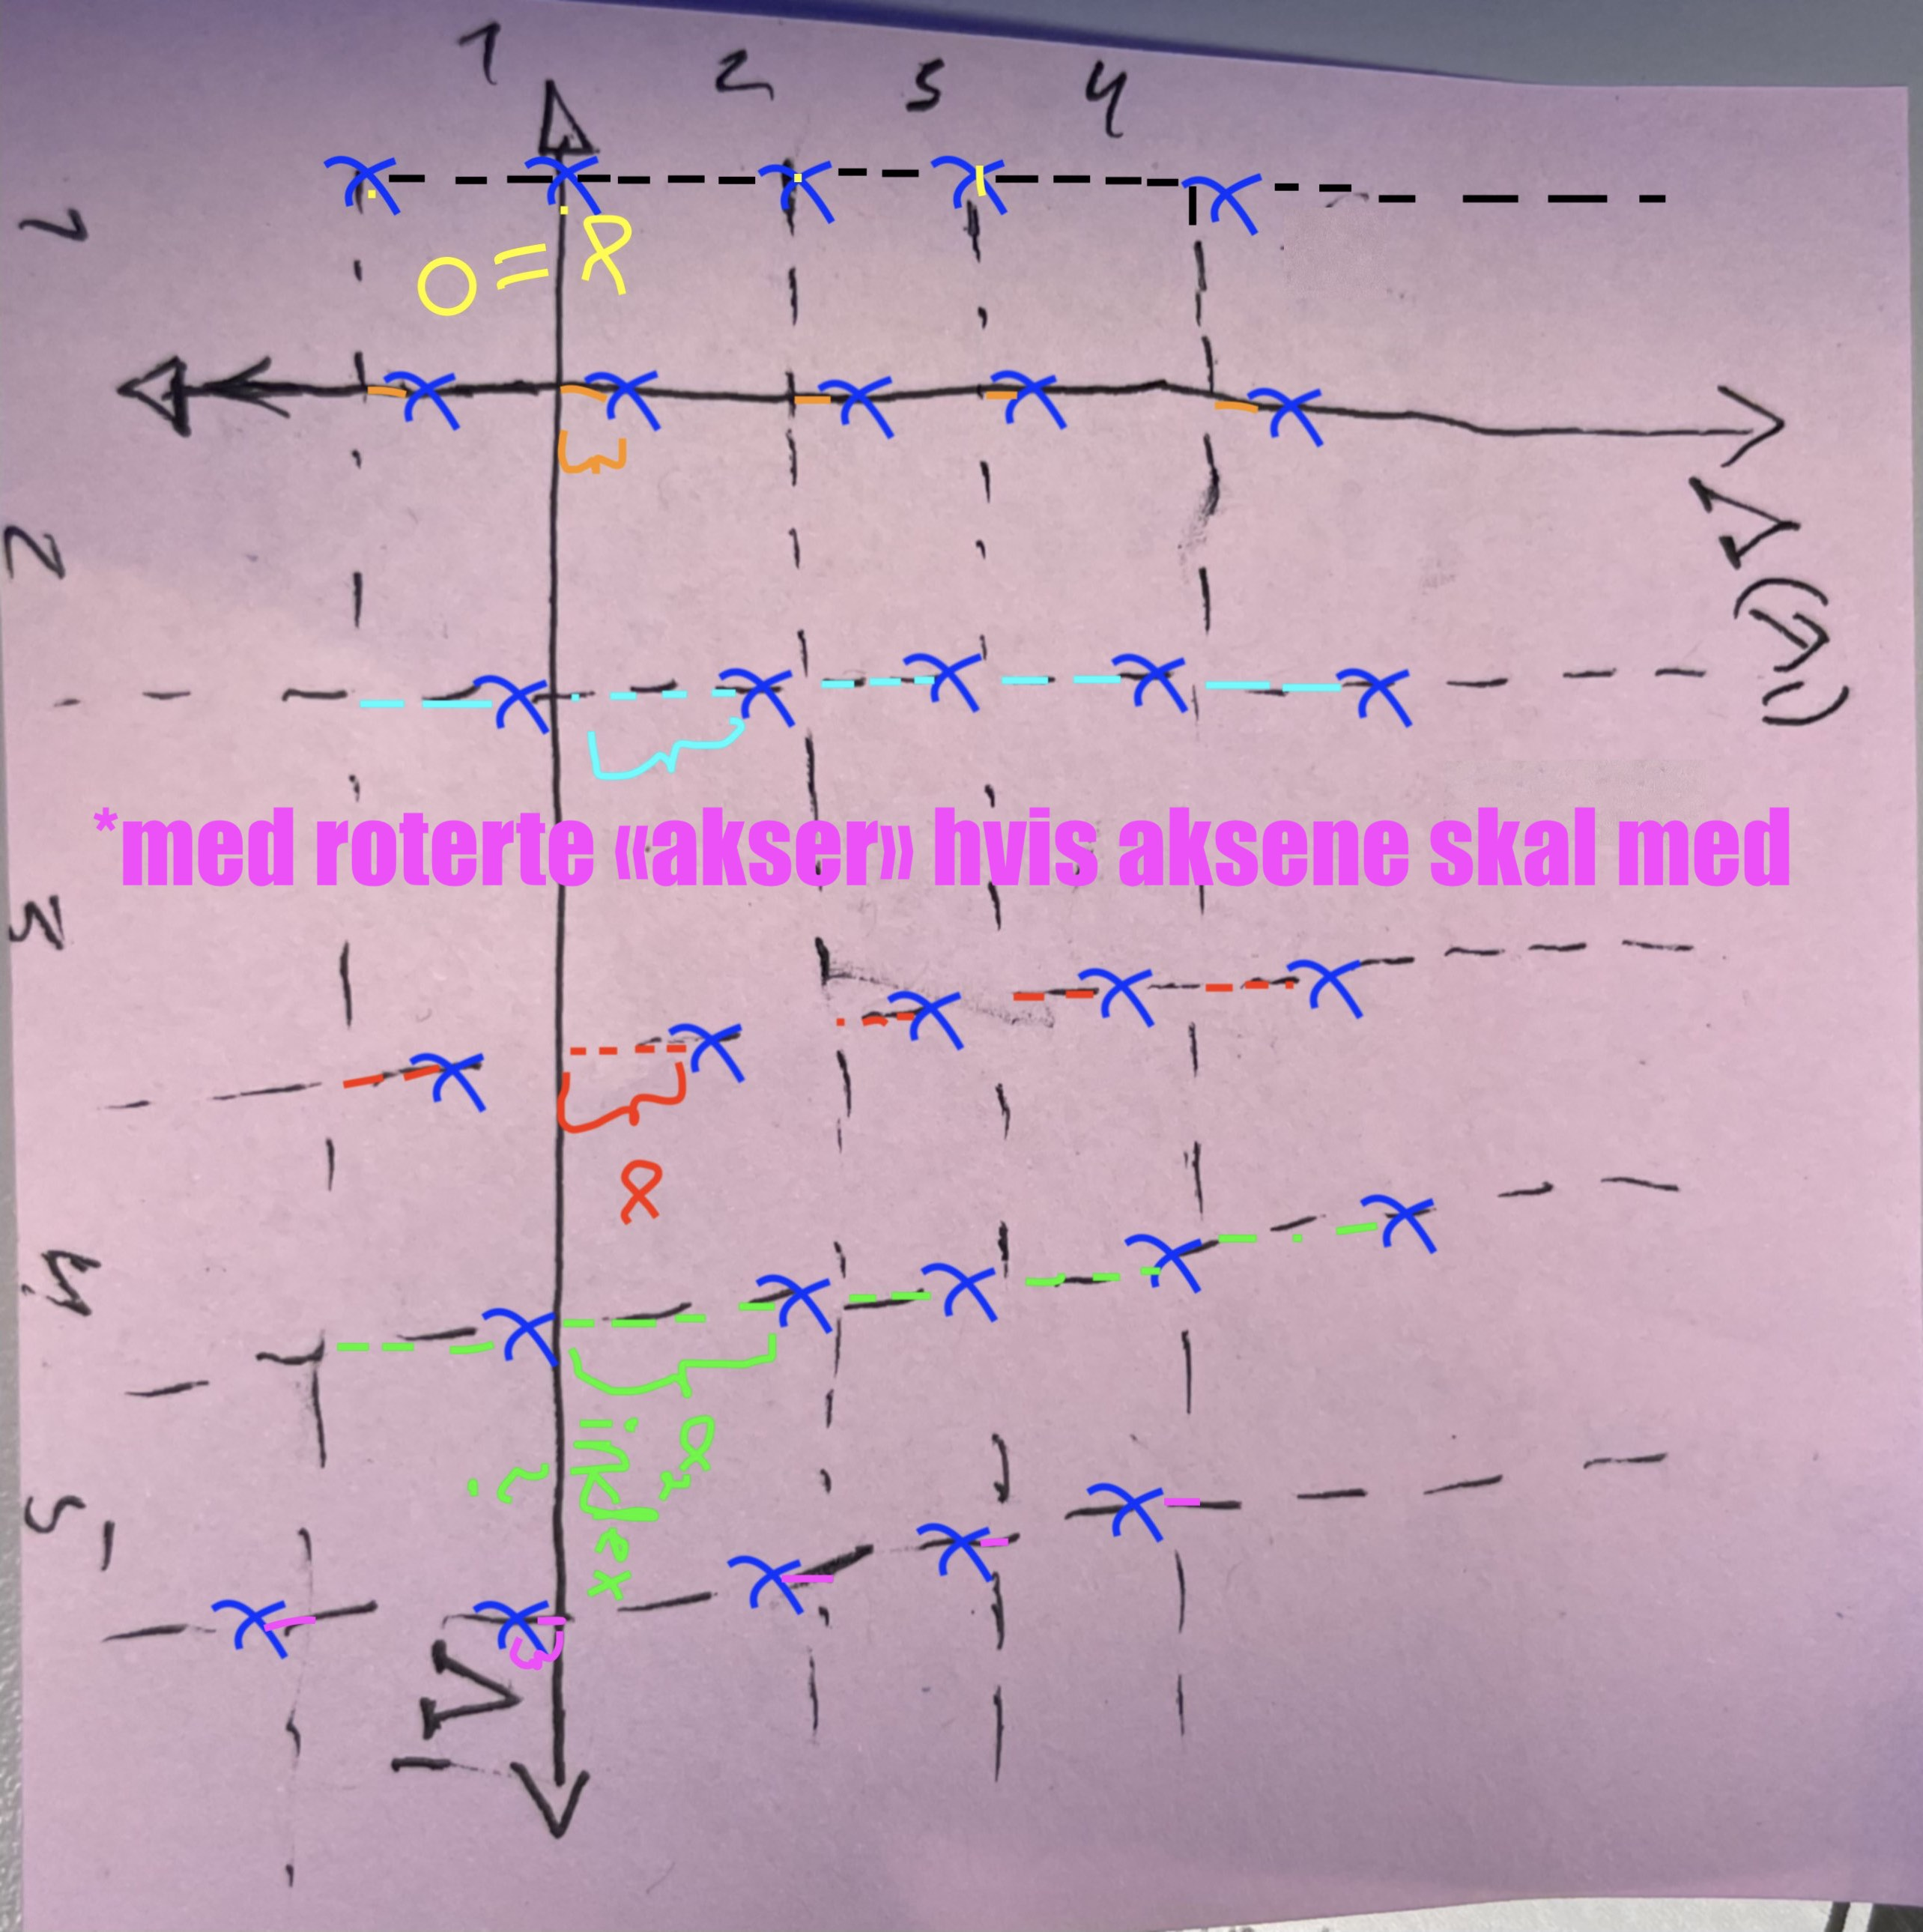
\includegraphics[width=0.9\linewidth]{multiple_shift_left_zero_horizontal.jpg}
        \caption{Multiple individual shifts horizontal}
        \label{fig:multiple_shift_horizontal}
    \end{subfigure}
    \caption{Illustration of the following pair of spectral pairs. In \labelcref{fig:lattice_spectra} we have $\brac{I,\Z}$ and $\brac{I,\lambfunc}$.  In \labelcref{fig:single_shift_vertical} we have $\brac{I,\Z}$ and $\brac{I,\lambfunc}$, where $\lambfunc$ is given by \labelcref{eq:single_shift_vertical}. In \labelcref{fig:multiple_shift_vertical} we have $\brac{I,\Z}$ and $\brac{I,\lambfunc}$, where $\lambfunc$ is given by \labelcref{eq:multiple_shit_func}. In \labelcref{fig:multiple_shift_horizontal} we have $\brac{I,\Z+0.4}$ and $\brac{I,\lambfunc}$, where $\lambfunc$ is given by \labelcref{eq:multiple_shit_func}.}
    \label{fig:spectra_figures}
\end{figure}


\SigridComment{ BEGYN HER MAX}
\begin{lemma}\label{lem:beta_shift}
    Let $\brac{\Omega_1,\Lambda_1}$ and $\brac{\Omega_2,\Lambda_2}$ be spectral pairs in dimensions $d_1$ and $d_2$ respectivly. Furthermore, define an arbitrary function $\betafunc: \Lambda_1 \rightarrow \R^{d_2}$, and let
    % $\betafunc: \Lambda_1 \rightarrow \R^{d_2}$ to denote the shift in the spectrum for $\Omega_2$ at each $\lambda_1$-value, and let %* unødvendig?
    \begin{equation}
        \Lambda = \Lambda_\beta
        = \braqMed{\begin{pmatrix}
            \lambda_1 \\
            \lambda_2+\betafunc(\lambda_1)
            \end{pmatrix}
        : \lambda_1 \in \Lambda_1 \text{ and } \lambda_2 \in \Lambda_2}.
    \end{equation}
    Then $\brac{\Omega_1 \times \Omega_2,\Lambda_\beta}$ is a spectral pair in $d_1+d_2$ dimensions. 
\end{lemma}
\begin{proof}
    As we assumed that $\brac{\Omega_2,\Lambda_2}$ is a spectral pair, it follows directly from \cref{lem:spectrum_shift_is_spectrum} that $\brac{\Omega_2,\Lambda_2+\beta}$ is also a spectral pair for any $\beta \in \R^{d_2}$ (with elements populated by $\betafunc(\lambda_1)$)
\end{proof}
\begin{remark}
    We can also shift the spectrum for $\Omega_1$ by a vector $\alpha \in \R^{d_1}$, to obtain the spectrum 
    \begin{equation*}
        \Lambda = \Lambda_{\alpha,\beta} 
        = \braqMed{\begin{pmatrix}
            \lambda_1 +\alpha\\
            \lambda_2+\betafunc(\lambda_1)
            \end{pmatrix}
        : \lambda_1 \in \Lambda_1 \text{ and } \lambda_2 \in \Lambda_2}
    \end{equation*}
    for $\Omega_1 \times \Omega_2$.
\end{remark}
%! Her representerer "funksjonen" vi hadde over, både en plaserings funksjon på \lambda_1, i tillegg til å skifte spektrumet akk. her med en reel verdi 
%! Funksjonen beta, poppulerer vektoren beta med elementer som er gitt av funksjonen. 

\begin{example}
    For two spectral sets $\brac{\Omega_1,\Lambda_1}=\brac{I, \Z+\alpha}$ and $\brac{\Omega_2,\Lambda_2}=\brac{I, \Z}$ a direct application of \cref{lem:beta_shift} would imply that $\brac{I^2,\Lambda_{\alpha,\beta}}$ is a spectral pair where
    \begin{equation*}
        \Lambda_{\alpha,\beta} 
        = \braqMed{\begin{pmatrix}
            \lambda_1 +\alpha\\
            \lambda_2+\betafunc_2(\lambda_1)
            \end{pmatrix}
        : \lambda_1 \in \Z +\alpha \text{ and } \lambda_2 \in \Z}. \qedhere
    \end{equation*}
\end{example}


\begin{example}
    By repeated application of \cref{lem:beta_shift} it will follow that $\brac{\Omega,\Lambda}= \brac{I^d, \Lambda}$ is a spectral pair if $\Lambda$ is given by % where the spectrum $\Lambda$ is the set of points given by
    \begin{equation*}
        \begin{pmatrix}
            \lambda_1 +\alpha\\
            \lambda_2+\beta_2(\lambda_1)\\
            \lambda_3+\beta_3(\lambda_1,\lambda_2)\\
            \vdots\\
            \lambda_d+\beta_d(\lambda_1,\dots,\lambda_{d-1})\\
        \end{pmatrix}
    \end{equation*}
    where all the elements $\lambda_1, \dots, \lambda_d \in \Z$ and each $\beta_{i+1}:\Z^{i} \rightarrow [0,1)$ are fixed functions.
    %* Skriv om; It is clear that the modifications result from the permutation of the $d$ coordinates.
\end{example}

%As with \cref{prop:class_all_shift}, we can classify all spectra in dimension two as follows. This significant result was proven by Pedersen and Jorgensen in the same paper \cite{jorgensenSpectralPairsCartesian2001}. 
We can now classify all spectra in dimension two as follows (\cite{jorgensenSpectralPairsCartesian2001}). 

\begin{theorem}\label{thrm:class_all_shift_2d}
    %$\braq{\beta_m \in [0,1) : m \in \Z}$  %* ANDRE skrivemåten for beta_m
    %For a fixed value $\alpha \in \R$ and an infinite sequence $\brac{\beta_m}_{m\in \Z}$, $\beta_m \in [0,1)$,  %* gammel
    The only subsets $\Lambda \subset \R^2$ such that $\Lambda$ is a spectrum for $\Omega = I^2$ are either one of the two classes
    \begin{equation}\label{eq:2d_all_shift_class_1}
        \Lambda = \braqMed{
            \begin{pmatrix}
            \alpha + m\\
            \beta_m + n
            \end{pmatrix} : m,n \in  \Z
            }
    \end{equation}
    or
    \begin{equation}\label{eq:2d_all_shift_class_2}
        \Lambda = \braqMed{
            \begin{pmatrix}
            \beta_n + m\\
            \alpha + n
            \end{pmatrix} : m,n \in  \Z
            }
    \end{equation}
    where $\alpha \in \R$ is fixed and $\brac{\beta_m}_{m\in \Z}$ is an infinite sequence with $\beta_m \in [0,1)$.
    %! \SigridComment{ekskludert delen om at det også er et tiling set, det er vel hensiktsmessik og splitte disse opp, og komme tilbake til det i neste del, for å så komme med fulle og hele theorem 3.2.} 
\end{theorem}
%!remark on the half open interval\\
%!remark om hvorfor sequencen er essensiell i dette tilfellet for å klassifisere alle skiftene\\ %, samenlignet bare med bare noen random skift
%!remark om at vi ikke kan ha ulike skift i to retninger, skiftene i den ene retningen må være fiksert.\\



\begin{proof}
    It follows directly from \cref{lem:beta_shift} that both classes given by \labelcref{eq:2d_all_shift_class_1} and \labelcref{eq:2d_all_shift_class_2} make $\brac{I^2,\Lambda}$ a spectral pair. To show that there are no other possibilities for $\Lambda$, we will make use of the inclusion
    \begin{equation}\label{eq:inclusion_dim_2}
        \Lambda - \Lambda \subset \Zstroke_{I^2} \cup \braq{0}
    \end{equation}
    where the zero-set $\Zstroke_{I^2}$ given in \cref{lem:zero_set_jp_1_5} is
    \begin{equation}\label{eq:zeroset_dim_2}
        \Zstroke_{I^2} = \braqMed{z = \brac{z_1,z_2} \in \C^2 : \exists \space j \in \braq{1,2} \text{ such that } z_j \in \intnozero}.
    \end{equation}
    To begin, let $\brac{I^2,\Lambda}$ be a spectral pair, which we know also implies that $\Lambda$ satisfies \labelcref{eq:inclusion_dim_2}. In addition, let us assume that the zero-element $\brac{0,0}$ is in $\Lambda$, as we can always translate $\Lambda$ by one vector so that the zero-element is in $\Lambda$. Now, let $\lambda = \brac{\lambda_1,\lambda_2} \in \Lambda$. From \labelcref{eq:inclusion_dim_2} we must have
    \begin{equation*}%* sidelengs fordi vi ser på elementer som er implisert fra inklusjonen, uten noen antagelser på Lambda
        \brac{\lambda_1, \lambda_2} - \brac{0,0} \in \Zstroke_{I^2} \cup \braq{0} \Longrightarrow \brac{\lambda_1, \lambda_2} \in \Zstroke_{I^2} \cup \braq{0}
    \end{equation*}
    That is, $\Lambda \subset \Zstroke_{I^2} \cup \braq{0}$. This means that at least one of $\lambda_1$ or $\lambda_2$ must be a non-zero integer for every $\lambda \in \Lambda$. This argument greatly reduces the possibilities as at least one of $\lambda_1$ or $\lambda_2$ must be a non-zero integer. Assume the minimum, with the added assumption that the other is anything but an integer. Now, take another arbitrary distinct element $\lambda'$ from $\Lambda$ using the two latter assumptions established for elements of $\Lambda$, but with opposite assumptions than for $\lambda$. There are two possibilities to do this, so first take $\lambda_1$ and $\lambda_2'$ to be non-zero integers, and take $\lambda_2$ and $\lambda_1'$ to be non-integers. Then, using  \labelcref{eq:inclusion_dim_2} and the fact that both 
    \begin{align*}
        \brac{\underbrace{\lambda_1}_{\in \intnozero}-\underbrace{\lambda_1'}_{\notin \Z}} \notin \intnozero
        \quad \text{and} \quad
        \brac{\underbrace{\lambda_2}_{\notin \Z}-\underbrace{\lambda_2'}_{\in \intnozero}} \notin \intnozero
    \end{align*}
    we get that $\brac{\lambda-\lambda'} \notin \Zstroke_{I^2}$ which contradicts \labelcref{eq:inclusion_dim_2}. As such, we must have at least $\lambda_1'\in \Z$ for any element $\lambda'\in \Lambda$, since this implies $\brac{\lambda_1 - \lambda_1'}\in \intnozero$ and that $\brac{\lambda-\lambda'} \in \Zstroke_{I^2}$. We have, however, not excluded the possibility that $\lambda_2$, and hence also $\brac{\lambda_2 - \lambda_2'}$, must also be an integer.
    
    \SigridComment{stemmer denne siste setningen, eller kan man nå egentlig direkte argumentere for at elementene fra $\Lambda$ er heltall i begge "koordinater".} 
    
    To show this, take $\lambda_1,\lambda'_1 \in \Z$ (not $\intnozero$!), and let $\lambda_1 = \lambda'_1$. We need no assumptions on $\lambda_2$ and $\lambda'_2$. Recall that $\lambda,\lambda'$ are distinct points. Then, from \labelcref{eq:inclusion_dim_2} and the fact that $\brac{\lambda_1-\lambda'_1}\in \Z$ we must have $\brac{\lambda_2-\lambda_2'} \in \Z$. And not only that, but from
    \begin{equation*}
        \brac{\lambda_1-\lambda'_1,\lambda_2-\lambda'_2} = \brac{0,\lambda_2-\lambda'_2}\in \Zstroke_{I^2},
    \end{equation*}
    it follows that $\brac{\lambda_2- \lambda_2'} \in \intnozero$. Otherwise, we would allow for $\lambda_2-\lambda_2'=0$ which would imply that $\lambda=\lambda'$ and yield a contradiction on our assumption that $\lambda\neq\lambda'$. By interchanging the vector notation from row to column form, observe $\Lambda$ is, in fact, a subset given by \labelcref{eq:2d_all_shift_class_1} with $\alpha = 0$, $m = \lambda_1$ and $n = \lambda_2$, as we have shown $\lambda_1, \lambda_2 \in \Z$ for all $\lambda \in \Lambda$. Furthermore, we know from \cref{lem:onb_direct_subset} that we cannot have an orthonormal basis as a direct subset of another orthonormal basis, thus we must have equality, and we have that $\Lambda$ is given by \labelcref{eq:2d_all_shift_class_1}.

    Let us now go back a few steps, and consider the other possibility. That is, take $\lambda_1$ and $\lambda_2'$ to be non-integers, and take $\lambda_2$ and $\lambda_1'$ to be non-zero integers. Then, from the fact that both 
    \begin{align*}
        \brac{\underbrace{\lambda_1}_{\notin \Z}-\underbrace{\lambda_1'}_{\in \intnozero}} \notin \intnozero
        \quad \text{and} \quad
        \brac{\underbrace{\lambda_2}_{\in \intnozero}-\underbrace{\lambda_2'}_{\notin \Z}} \notin \intnozero
    \end{align*}
    we get that $\brac{\lambda-\lambda'} \notin \Zstroke_{I^2}$, and we must have at least $\lambda_2'\in \Z$ for any element $\lambda'\in \Lambda$. To exclude the possibility that $\lambda_1$ is an integer, take $\lambda_2,\lambda'_2 \in \Z$ and let $\lambda_2 = \lambda'_2$. Since we still have the assumtion that $\lambda, \lambda'$ are distinct points, then from \labelcref{eq:inclusion_dim_2} and the fact that $\brac{\lambda_1-\lambda'_1}\in \Z$ we must have $\brac{\lambda_2-\lambda_2'} \in \Z$. And not only that, but from
    \begin{equation*}
        \brac{\lambda_1-\lambda'_1,\lambda_2-\lambda'_2} = \brac{\lambda_1-\lambda'_1,0}\in \Zstroke_{I^2},
    \end{equation*}
    it follows that $\brac{\lambda_2- \lambda_2'} \in \intnozero$. Again, by interchanging the vector notation we get that $\Lambda$ is a subset of \labelcref{eq:2d_all_shift_class_2} with $\alpha = 0$, $m = \lambda_1$ and $n = \lambda_2$, as $\lambda_1, \lambda_2 \in \Z$ for all $\lambda \in \Lambda$. Using \cref{lem:onb_direct_subset} we get that it cannot be a subset given by \labelcref{eq:2d_all_shift_class_2}, and we must have equality.

    We now have established that $\brac{I^2, \Lambda}$ is a spectral pair in the case where $\Lambda$ is given by either \labelcref{eq:2d_all_shift_class_1} or \labelcref{eq:2d_all_shift_class_2} and that there are no other spectra for $I$ in dimension $d=2$. 


    %* dette er det vi viser heelt til slutt
    %, and if the other element is the non-zero element, then at least one of $\lambda_1,\lambda_2$ must be non-zero. 

    %* sistebiten, kanskje nyttig
    % Now, we must also verify that $\Lambda$ must be a subset of a set given by \labelcref{eq:2d_all_shift_class_1}, and also exclude the possibility that $\brac{\lambda_2 - \lambda_2'}$ is not an integer (not necessarily a non-zero one).
\end{proof}



\end{document}